\section{Method}
% SD 状态切换示意图
\begin{figure}[t]
    \vspace{-20pt}
    \begin{center}
    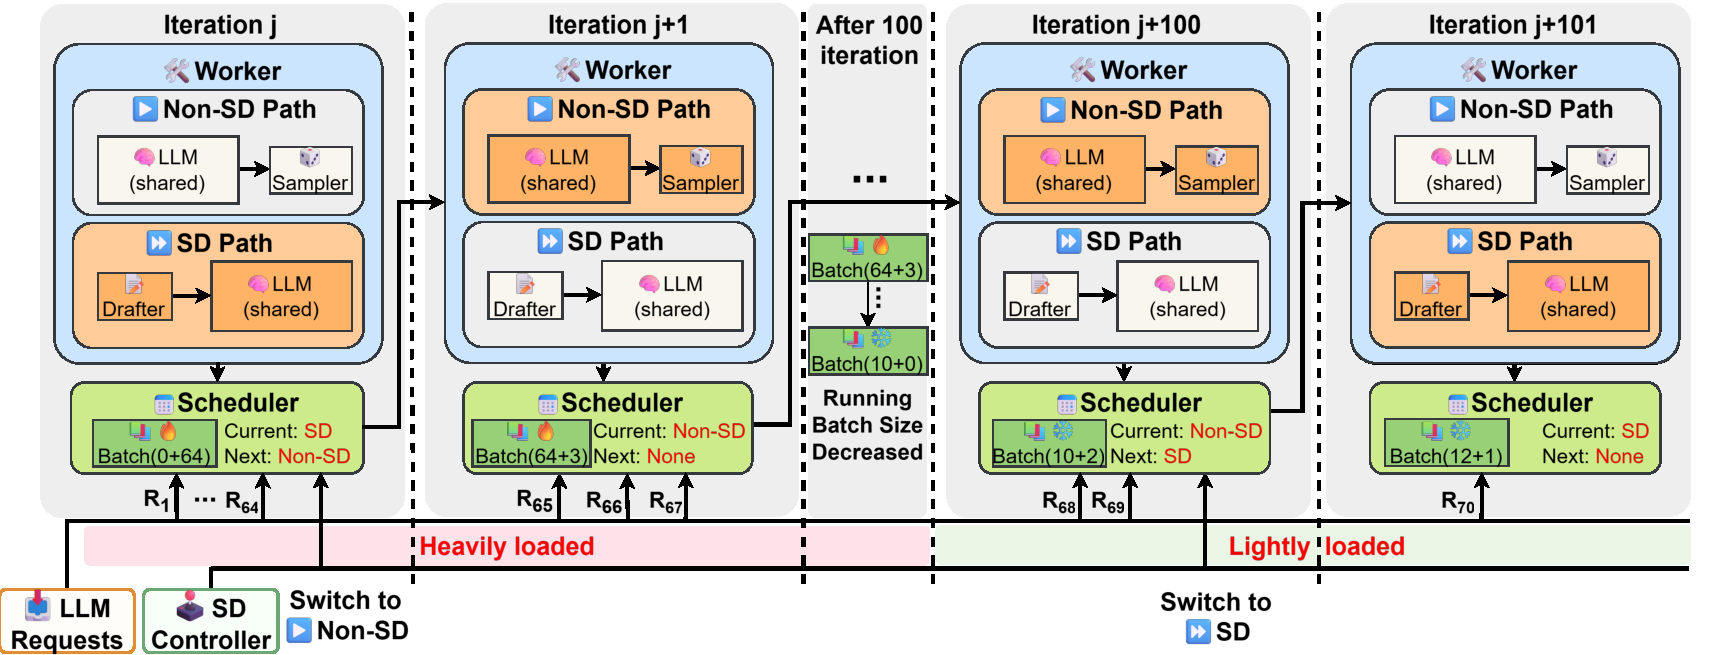
\includegraphics[width=1.0\linewidth]{figures/method-overview.pdf}
    \end{center}
    \vspace{-10pt}
    % \caption{
    %     Illustration of iteration-level SD switching in \sysname.
    %     At iteration $i$, a heavily loaded batch triggers a \emph{Switch to Non-SD} request, which is forwarded by the scheduler and takes effect at iteration $i+1$.
    %     Similarly, a \emph{Switch to SD} request issued under light load at iteration $i+2$ takes effect at iteration $i+3$.
    %     All requests within an iteration follow the same execution mode.
    % }
    \caption{
    Illustration of iteration-level SD switching in \sysname.
    At iteration $j$, 64 incoming requests drive the system into a heavily loaded state, causing the external SD Controller to issue a switch-to-Non-SD request.
    The internal Scheduler applies the request at iteration $j+1$, and inference proceeds along the native Non-SD path for the next 100 iterations as the running batch size gradually decreases.
    After the system becomes lightly loaded, the SD Controller issues a switch-to-SD request, which takes effect at iteration $j+101$, after which inference continues along the native SD path.
    }
    \label{fig:sd_switch}
\end{figure}

% 1.支持 SD 动态切换的外部接口
\subsection{Externally Controllable SD Switching}
\label{sec:4.1}
% 总起，分成三部分：外部接口，scheduler，worker
% To support customizable SD selection policies at the upper layer, \sysname extends the underlying inference engine with an externally controllable runtime SD switch  \xiaoxi{emphasize the existing dynamic SD pre-sets a static switching condition, and more importantly, their default path is fixed to the SD Path, resulting a xxxx overhead.}.


Existing dynamic SD approaches have two limitations. First, their switching logic is embedded within the inference engine, limiting customized upper-layer control. Second, disabling SD does not necessarily restore the native non-SD path: %their non-SD mode is still confined to the SD path, %retaining substantial residual overhead. 
% as shown in~\autoref{tab:token_consistency_form} and~\autoref{fig:nonsd_overhead_b32}.
as shown in~\autoref{tab:token_consistency_form}, vLLM Dynamic SD (vLLM-DSD) and SGLang Adaptive SD (SGLang-ASD) with zero draft length remain token-consistent with native SD but not with native Non-SD, indicating that they still follow the SD path 
(detailed in~\autoref{dynamic-sd-comparison}). %The resulting overhead is shown in~\autoref{fig:nonsd_overhead_b32}.
\sysname %exposes an externally controllable runtime interface that 
addresses these issues by decoupling mode selection logic from engine execution and switching directly between native SD and non-SD paths, significantly reducing non-SD overhead (see~\autoref{fig:nonsd_overhead_b32}). As shown in~\autoref{fig:sd_switch}, this design consists of three components: %an external control interface, an iteration-level state transition in the scheduler, and path-specific execution paths in the worker (Figure~\autoref{fig:sd_switch}).
% \xiaoxi{Please change the description of Figure~\ref{fig:sd_switch} to the phenomenon/benefit of switching.} 

% \xiaoxi{Move Table~\ref{tab:token_consistency} and Figure~\ref{fig:nonsd_overhead} here in a compact way.}


% 描述 existing dynamic SD 方法的问题：没有彻底切换，存在overhead
\begin{figure}[b]
    \vspace{-10pt}
    \centering
    % =========================
    % Left: Table
    % =========================
    \begin{minipage}[t]{0.73\linewidth}
        \centering
        \captionof{table}{Token consistency across adaptive SD approaches.}
        \label{tab:token_consistency_form}
    
        \resizebox{\linewidth}{!}{
        \begin{tabular}{cccc}
            \toprule
            \textbf{Inference Engine} &
            \textbf{Approach} &
            \textbf{Non-SD} &
            \textbf{SD} \\
            \midrule
    
            \multirow{3}{*}{vLLM}
            & Dynamic SD ($\text{draft\_len}=0$)
            & $\times$ & $\checkmark$ \\
    
            & SpecSys-NonSD
            & $\checkmark$ & -- \\
    
            & SpecSys-SD
            & -- & $\checkmark$ \\
    
            \midrule
    
            \multirow{3}{*}{SGLang}
            & Adaptive SD ($\text{draft\_len}=0$)
            & $\times$ & $\checkmark$ \\
    
            & SpecSys-NonSD
            & $\checkmark$ & -- \\
    
            & SpecSys-SD
            & -- & $\checkmark$ \\
    
            \bottomrule
        \end{tabular}
        }
    \end{minipage}
    \hfill
    % =========================
    % Right: Figure
    % =========================
    \begin{minipage}[t]{0.26\linewidth}
        \vspace{0pt}
        \centering
        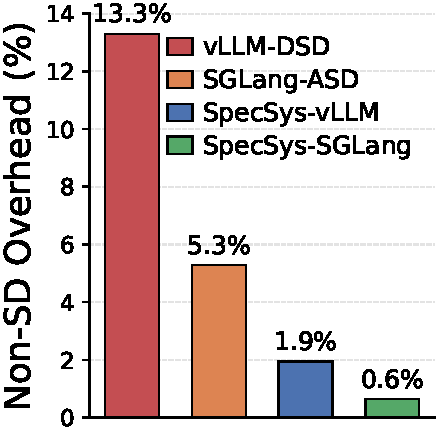
\includegraphics[width=\linewidth]{figures/nonsd_overhead_bs32.pdf}
        \setlength{\abovecaptionskip}{-15pt}
        \captionof{figure}{Non-SD Path Overhead of Adaptive SD}
        \label{fig:nonsd_overhead_b32}
    \end{minipage}

\end{figure}


% 外部接口
\textbf{External Control Interface.}
% \sysname extends the inference engine with a lightweight control interface to receive SD switching requests and forward them to the scheduler to update the desired execution mode.
% This design decouples the external scheduling policy from the internal execution logic of the inference engine. \xiaoxi{still need to highlight the fundamental benefit, e.g., improved deployment flexibility or extendibility}
\sysname exposes a lightweight control interface that receives SD switching requests and forwards them to the scheduler to update the desired execution mode.
This design decouples the switching policy from internal execution logic, allowing customized policies to be changed or replaced without modifying the underlying inference engine.
%As a result, \sysname can be flexibly integrated with different deployment environments and external scheduling strategies.

% scheduler
\textbf{Iteration-Level State Transition.}
% To ensure execution consistency, \sysname performs SD switching only at inference-iteration boundaries \xiaoxi{A better way to highlight our method that enables iteration-level switching should be relating this iteration-level switching to the purpose of reducing JCT in addition to execution consistency}. 
%To eliminate the lag between external control and internal execution introduced by this decoupled design, \sysname adopts iteration-level switching, allowing switching requests to take effect at the next inference iteration.
%Specifically, the scheduler maintains a current mode and an expected mode. External requests update only the expected mode, which is applied to the worker at the next iteration boundary.
Serving conditions can change while a continuous batch remains active, so coarse-grained reconfiguration may delay a needed switch. \sysname therefore applies mode changes at inference-iteration boundaries, so controller decisions take effect at the next iteration without disrupting the current one. The scheduler tracks current and next modes; external requests update the next mode, which is then propagated to the worker.

% worker
\textbf{Path-Specific Worker Execution.}
% As Non-SD and SD follow different execution paths (in~\autoref{sec:3.1}), \sysname preserves separate execution branches for the two paths. 
% During engine initialization, CUDA Graphs for both modes are prepared in advance. \xiaoxi{Should point out the importance or challenging issue related to CUDA graphs in the switching.}
% At runtime, the worker selects the corresponding execution branch and CUDA Graph based on the mode specified in \texttt{SchedulerOutput}. 
% Within each iteration, all requests in the batch follow the same execution mode and therefore share the same execution path, ensuring consistent batch execution while enabling low-overhead iteration-level switching.
Existing dynamic SD approaches focus on the SD path and provide limited optimization for native Non-SD execution, especially dedicated CUDA Graphs. Extending switching to two native paths therefore requires optimizing both paths independently. 
\sysname prepares CUDA Graphs for both paths during initialization, and the worker uses the pre-captured CUDA Graph corresponding to the selected path in each iteration.



% 2.Agent 剩余 step 数预测
\subsection{Agent Remaining-Step Prediction}
\label{sec:4.2}
% 介绍预测方法的动机
% \xiaoxirev{To realize an efficient scheduling mechanism that exploits unique characteristics of agent workloads, we conduct a profiling experiment
% %Based on our profiling results 
% (\autoref{step-distribution}), which reveals two insights}: {\em (i) Agent execution patterns vary across workflows and workloads. (ii) The prompts of LLM inference steps provide useful information of the current execution state that can guide scheduling decisions}. 
% First, we categorize today's agent workflows into three types:

% \xiaoxi{cite references below, for the workflow terminologies that appear in the first time}
% \begin{itemize}[leftmargin=10pt]
%     \item \textbf{Type A} represents planning-based workflows, such as Plan-and-Solve, where the planned step count can be directly extracted from the prompt, making prediction straightforward.
%     \item \textbf{Type B} represents multi-step iterative workflows, such as AgentFlow, where tasks terminate at specific step boundaries and exhibit a multimodal step distribution, making the completion step easier to estimate using the mode of the historical distribution.
%     \item \textbf{Type C} represents step-by-step workflows, such as ReAct, where tasks may terminate at almost any step, making prediction more difficult and requiring additional execution-state information.
% \end{itemize}
To exploit agent-specific execution patterns for remaining-step prediction, we profile representative agent workflows and categorize them into three types:
%To realize an efficient scheduling mechanism that exploits unique characteristics of agent workloads, we conduct a profiling experiment
%Based on our profiling results 
%(\autoref{step-distribution}), which reveals two insights: {\em (i) Agent execution patterns vary across workflows and workloads. (ii) The prompts of LLM inference steps provide useful information of the current execution state that can guide scheduling decisions}. 
%First, we categorize today's agent workflows into three types:

% \begin{itemize}[leftmargin=10pt]\label{type-describe}
%     \item \textbf{Type A} represents planning-based workflows, such as Plan-and-Solve, where the planned step count can be directly extracted from the \xiaoxirev{planning output}, making prediction straightforward.
%     \item \textbf{Type B} represents multi-step iterative workflows, such as AgentFlow, where tasks terminate at specific step boundaries and exhibit a multimodal step distribution, making the completion step easier to estimate using the mode of the historical distribution.
%     \item \textbf{Type C} represents step-by-step workflows, such as ReAct, where tasks may terminate at almost any step, making prediction more difficult and requiring additional execution-state information.
% \end{itemize}

\begin{itemize}[leftmargin=10pt]\label{type-describe}
    \item \textbf{Type A} represents planning-based workflows, such as Plan-and-Solve, where the planned step count can be extracted from the planning output. %, making prediction straightforward. 
    A parsing example is provided in~\autoref{prompt_parser}.
    \item \textbf{Type B} represents multi-step iterative workflows, such as AgentFlow, where tasks terminate at specific step boundaries and exhibit a multimodal step distribution (see~\autoref{step-distribution}), enabling completion-step  estimation from historical distributions.
    \item \textbf{Type C} represents step-by-step workflows, such as ReAct, where tasks may terminate at almost any step, requiring additional execution-state information for prediction.
\end{itemize}
Across these workflow types, our profiling identifies two complementary signals for remaining-step prediction: historical execution patterns conditioned on workflow and workload, and execution-state cues exposed by the current LLM-call prompt.

% 解析请求附带的信息，提取状态关键词，然后分类。
\textbf{Request-Level Information Extraction.}
For each LLM request, the upstream agent application provides its workflow, workload, and current execution step as metadata. 
\sysname further parses the prompt for keywords indicating {\em errors, repeated actions, completion, and termination}, and maps the request to a workflow-specific {\em execution state}.
Concrete examples are provided in~\autoref{prompt_parser}.

% 分类保存历史记录
\textbf{Offline History Profiling.}
% \sysname groups completed agent requests by workflow and workload and records the distribution of total execution steps $T$. 
% The distributions are further conditioned on the extracted execution state and, for Type C workflows, the transition between the previous and current states. \xiaoxi{mention the profiling cost is not large.}
\sysname groups completed agent requests by workflow and workload and records the distribution of total execution steps $T$. 
The distributions are further conditioned on the extracted execution state and, for Type C workflows, the transition between the previous and current states.
The profiling cost is negligible, as \sysname only maintains lightweight statistics over completed requests and performs no additional computation on the online serving path.

% \xiaoxi{Please explain the reason/intuition of each specific way/parameter used in the following estimation for different workflow types. Make them tightly related to your observations.}

% 剩余 step 数估计
\textbf{Remaining-Step Estimation.}
% todo: 解释一下为什么要用这样的方法
%\sysname adopts different estimation strategies based on the characteristics of each workflow type as described in~\autoref{type-describe}.
For each workflow type, \sysname estimates the remaining steps using workflow-specific signals. Let $\hat{R}_x$ denote the estimate for Type $x$. Type A leverages the explicit plan; Type B uses the most frequent historical completion step to capture recurring termination patterns; Type C further incorporates state transitions and uses the median for more robust estimation.

% Type A，解析 plan 直接得到 P ，然后 P-k 得到剩余 step
For \textbf{Type A}, let $P$ denote the planned step count extracted from the prompt. 
Given the current step $k$, the remaining steps are directly computed as
\begin{equation}
\hat{R}_{A} = \max(0, P-k).
\end{equation}

% Type B，看当前状态，根据对应的分类槽里的历史信息中的条件众数得到预测结果
For \textbf{Type B}, let $s_k$ denote the execution state at step $k$. 
\sysname estimates the completion step using the mode of the historical distribution conditioned on the current step and execution state:
\begin{equation}
\hat{T}_{B} =
\mathrm{mode}\{T \mid k, s_k\},
\qquad
\hat{R}_{B} = \max(0, \hat{T}_{B}-k).
\end{equation}

% Type C，看当前状态+历史状态，根据对应的分类槽里的历史信息中的条件中位数得到预测结果
For \textbf{Type C}, \sysname further conditions the historical records on both the previous state $s_{k-1}$ and current execution state $s_k$ and uses the median of the corresponding historical distribution:

\begin{equation}
\hat{T}_{C} =
\mathrm{median}\{T \mid k, s_{k-1}, s_k\},
\qquad
\hat{R}_{C} = \max(0, \hat{T}_{C}-k).
\end{equation}

When the fine-grained statistics are insufficient, \sysname progressively falls back to the current-state-conditioned distribution and then to the workflow-workload-level historical distribution.


% 3.基于动态负载的 Agent 任务调度和 SD 选择
\subsection{Load-Adaptive Agent Scheduling and SD Selection}
\label{sec:4.3}

% 离线 profile 出不同配置下的 SD加速比与推理负载的关系，得到一个平衡点。
\textbf{Offline SD Speedup Profiling.}
\label{sec:4.3.1}
For each model and hardware configuration, \sysname profiles SD speedup across different batch sizes before engine startup and identifies the break-even load $B^{*}$, defined as the largest batch size at which SD achieves a speedup greater than or equal to 1. 
SD is beneficial below $B^{*}$, while its overhead can cause performance degradation above this point. Detailed profiling results are provided in~\autoref{sd-speedup}.

% 负载估计
\textbf{Future-Load Estimation.}
% 因为切换存在一定的滞后性。考虑负载时不仅是看推理引擎内部的running batch size，还要看外部proxy的计划resume的任务数，二者相加得到预测的未来负载。
Since SD switching takes effect with a short delay, the current running batch size alone may not reflect the load when the new mode becomes active. 
\sysname therefore also considers agent requests temporarily held by the router-proxy that are scheduled to be resumed and submitted to the inference engine. 
Specifically, it estimates the near-future load by combining the current running batch size $B_{\mathrm{running}}$ with the number of requests to be resumed $B_{\mathrm{resume}}$:
\begin{equation}
\hat{B}=B_{\mathrm{running}}+B_{\mathrm{resume}}.
\end{equation}

% 基于负载选择性使用SD
\textbf{Load-Adaptive SD Selection.}
\sysname compares the estimated load $\hat{B}$ with the profiled break-even load $B^{*}$ and sends an SD-switching request to the inference engine interface accordingly. The SD execution mode is determined as
\begin{equation}
\mathrm{Enable\mbox{-}SD} =
\begin{cases}
\mathrm{True},  & \hat{B} \leq B^{*}, \\
\mathrm{False}, & \hat{B} > B^{*}.
\end{cases}
\end{equation}
This strategy enables SD under low load to mitigate the decode bottleneck.

% 高负载下的任务调度策略
\textbf{Agent Task Scheduling.}
When the serving load becomes high and agent tasks start queuing at the router-proxy, \sysname prioritizes the task with the fewest predicted remaining steps:
\begin{equation}
j^{*} =
\operatorname*{arg\,min}_{j \in \mathcal{Q}}
\hat{R}_{j},
\end{equation}
where $\mathcal{Q}$ denotes the queued agent tasks and $\hat{R}_{j}$ is the remaining steps of task $j$ estimated by the predictor in~\autoref{sec:4.2}.
This strategy prioritizes tasks closer to completion, thereby mitigating the queue bottleneck under high serving load.